\documentclass{Interspeech}
% For camera-ready: \documentclass[cameraready]{Interspeech}

\usepackage{amsmath,amssymb}
\usepackage{booktabs}
\usepackage{tikz}
\usetikzlibrary{positioning,arrows.meta,fit,calc}
\usepackage{pgfplots}
\pgfplotsset{compat=1.18}
\usepackage{multirow}
\usepackage{xcolor}
\usepackage{bm}

\title{NanoMamba: Noise-Robust Keyword Spotting with \\ Spectral-Aware State Space Models}

% Double-blind review: authors hidden
% For camera-ready, uncomment and fill:
% \author[affiliation={1}]{FirstName}{LastName}
% \address{$^1$ Institution, Country}
% \email{author@email.com}

\keywords{keyword spotting, state space model, noise robustness, edge AI}

\begin{document}
\maketitle

% ============================================================
% ABSTRACT
% ============================================================
\begin{abstract}
Keyword spotting (KWS) on edge devices demands ultra-small models, yet noise robustness typically requires additional parameters for denoising.
We propose NanoMamba, a KWS architecture built on Spectral-Aware State Space Models (SA-SSM) that dynamically modulates SSM dynamics based on per-band SNR estimates.
SA-SSM adjusts the discretization step~$\Delta$ and input matrix~$\mathbf{B}$ in response to estimated noise conditions, enabling inherent noise adaptation without a separate denoising front-end.
On Google Speech Commands~V2 (12-class), NanoMamba-Small (12K~parameters, 11.8\,KB INT8) achieves 95.1\% test accuracy---within 1.3 percentage points of DS-CNN-S (24K~parameters)---while retaining 84.5\% of clean accuracy at 0\,dB noise versus 55.2\% for DS-CNN-S.
Under broadband white noise at 0\,dB, NanoMamba-Small maintains 83.9\% versus 13.9\% for DS-CNN-S, revealing catastrophic failure of fixed-filter CNN architectures under spectrally uniform noise.
\end{abstract}

% ============================================================
% 1. INTRODUCTION
% ============================================================
\section{Introduction}

Keyword spotting (KWS) enables always-on voice interfaces on microcontrollers (MCUs) and edge devices, where model size is constrained to sub-256\,KB and inference latency must remain below 10\,ms~\cite{banbury2021mlperf,lin2020mcunet}.
Recent architectures such as BC-ResNet~\cite{kim2021bcresnet} and DS-CNN~\cite{zhang2017hello} achieve high clean accuracy with small footprints, yet they lack explicit mechanisms for noise adaptation---performance degrades substantially under real-world noise conditions such as factory floors, street traffic, or multi-talker environments.

State space models (SSMs), particularly Mamba~\cite{gu2024mamba}, have emerged as efficient alternatives to Transformers for sequential modeling, offering linear-time complexity and constant memory during inference.
Keyword Mamba~\cite{goel2024keyword} demonstrated that SSMs can achieve state-of-the-art KWS accuracy, but with 3.4M parameters---far exceeding edge deployment budgets.
Moreover, no prior work has explored \emph{noise-aware modulation} of SSM dynamics for KWS.

We propose \textbf{NanoMamba}, an ultra-compact KWS architecture that introduces \textbf{Spectral-Aware SSM (SA-SSM)}, where the SSM discretization step~$\Delta$ and input matrix~$\mathbf{B}$ are dynamically modulated by per-band SNR estimates.
Our contributions are:
\begin{itemize}
\setlength\itemsep{0pt}
\item SA-SSM: a noise-aware SSM mechanism that adjusts $\Delta$ (state dynamics speed) and $\mathbf{B}$ (input gating) based on real-time SNR estimation, enabling inherent noise robustness without a separate denoising module.
\item NanoMamba: a family of ultra-compact KWS models (4,636--12,035 parameters; 4.5--11.8\,KB in INT8) that significantly outperform CNN baselines under noise while achieving competitive clean accuracy, demonstrating that noise robustness need not come at the cost of model size.
\end{itemize}

% ============================================================
% 2. PROPOSED METHOD
% ============================================================
\section{Proposed Method}

\subsection{Theoretical Background}
\label{sec:theory}

\smallskip\noindent\textbf{SSM discretization and frequency selectivity.}
Under zero-order hold (ZOH) discretization, the continuous SSM parameters $(A, B)$ are mapped to discrete counterparts $\bar{A} = \exp(A \Delta)$ and $\bar{B} = \Delta \cdot B$.
When $\Delta \to 0$, $\bar{A} \to I$ and $\bar{B} \to 0$, so the state $\mathbf{h}_t \approx \mathbf{h}_{t-1}$ and external input is suppressed.
In frequency-domain terms, the discrete SSM transfer function
\begin{equation}
H(z) = \mathbf{C}(z\mathbf{I} - \bar{\mathbf{A}})^{-1}\bar{\mathbf{B}} + \mathbf{D}
\label{eq:transfer}
\end{equation}
exhibits a bandwidth proportional to $\Delta$: smaller $\Delta$ concentrates the passband at low frequencies, effectively acting as a \emph{low-pass filter} that suppresses high-frequency noise components.
Conversely, larger $\Delta$ widens the bandwidth, preserving temporal detail in clean signals.
This motivates SNR-conditioned control of $\Delta$: reduce $\Delta$ under noise to filter transients, and increase $\Delta$ under clean conditions to retain signal fidelity.

\smallskip\noindent\textbf{Input gating as Bayesian state estimation.}
The SSM state update $\mathbf{h}_t = \bar{\mathbf{A}}\mathbf{h}_{t-1} + \bar{\mathbf{B}}x_t$ can be viewed as a Bayesian estimator where $\bar{\mathbf{A}}\mathbf{h}_{t-1}$ is the \emph{prior} (predicted state) and $\bar{\mathbf{B}}x_t$ is the \emph{observation} (new evidence from input).
In high-noise conditions, the observation $x_t$ is unreliable.
A rational strategy is to trust the prior and attenuate the observation:
\vspace{-2pt}
\begin{equation}
\tilde{\mathbf{B}} \to 0 \quad\Longrightarrow\quad
\mathbf{h}_t = \bar{\mathbf{A}}\,\mathbf{h}_{t-1} + \tilde{\mathbf{B}}\,x_t
\approx \bar{\mathbf{A}}\,\mathbf{h}_{t-1}.
\label{eq:bayesian}
\end{equation}
This is precisely what B-gating achieves: when SNR is low, $\tilde{\mathbf{B}} \to 0$, preserving accumulated state memory while rejecting noisy input.

\smallskip\noindent\textbf{Per-band vs.\ global SNR adaptation.}
Real-world noise exhibits frequency-dependent structure: factory noise concentrates energy below 500\,Hz, babble noise overlaps the speech formant range (300--3000\,Hz), while white noise is spectrally flat.
A global SNR estimate collapses this structure into a single scalar, losing band-specific information.
Per-band SNR estimation provides a vector $\hat{\mathbf{s}}_t \in \mathbb{R}^F$, enabling the model to selectively suppress noisy bands while preserving clean ones---analogous to a learned, time-varying Wiener filter~\cite{haykin2014adaptive} integrated directly into the SSM dynamics.

\subsection{NanoMamba Architecture}

Figure~\ref{fig:arch} illustrates the NanoMamba architecture.
Given a 1-second audio input at 16\,kHz, we compute a magnitude spectrogram via STFT (512-point FFT, 160-sample hop, 400-sample Hann window) and derive two parallel representations:
(1)~a 40-band log-mel spectrogram $\mathbf{X} \in \mathbb{R}^{B \times F \times T}$ as input features, and
(2)~per-band SNR estimates $\hat{\mathbf{s}} \in \mathbb{R}^{B \times F \times T}$ from the SNR Estimator.

The mel features are projected to dimension $d$ via a linear layer and processed by $L$ stacked SA-SSM blocks.
Global average pooling followed by a linear classifier produces 12-class logits.

\begin{figure}[t]
\centering
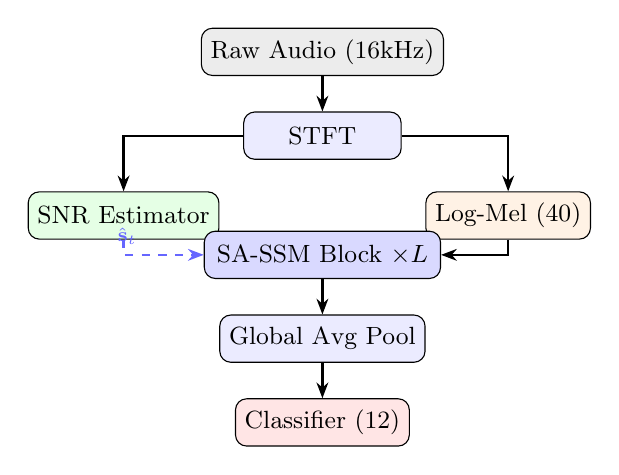
\begin{tikzpicture}[
    block/.style={draw, rounded corners, minimum height=0.6cm, minimum width=2.0cm, font=\small, fill=blue!8},
    arrow/.style={-{Stealth[length=2mm]}, thick},
    label/.style={font=\scriptsize},
    node distance=0.45cm
]
% Input
\node[block, fill=gray!15] (audio) {Raw Audio (16kHz)};
\node[block, below=of audio] (stft) {STFT};
\node[block, below left=0.4cm and 0.3cm of stft, fill=green!10] (snr) {SNR Estimator};
\node[block, below right=0.4cm and 0.3cm of stft, fill=orange!10] (mel) {Log-Mel (40)};
\node[block, below=0.9cm of stft, fill=blue!15, minimum width=3.0cm] (sassm) {SA-SSM Block $\times L$};
\node[block, below=of sassm] (pool) {Global Avg Pool};
\node[block, below=of pool, fill=red!10] (cls) {Classifier (12)};

% Arrows
\draw[arrow] (audio) -- (stft);
\draw[arrow] (stft) -| (snr);
\draw[arrow] (stft) -| (mel);
\draw[arrow] (mel) |- (sassm);
\draw[arrow, dashed, blue!60] (snr) |- node[label, above left, xshift=0.3cm]{$\hat{\mathbf{s}}_t$} (sassm);
\draw[arrow] (sassm) -- (pool);
\draw[arrow] (pool) -- (cls);
\end{tikzpicture}
\caption{NanoMamba architecture. Dashed line indicates SNR conditioning of SA-SSM dynamics.}
\label{fig:arch}
\end{figure}

\subsection{Spectral-Aware SSM (SA-SSM)}

A standard selective SSM~\cite{gu2024mamba} processes a 1-D input sequence $x_t \in \mathbb{R}^D$ via:
\begin{align}
\mathbf{h}_t &= \bar{\mathbf{A}} \, \mathbf{h}_{t-1} + \bar{\mathbf{B}} \, x_t, \quad
y_t = \mathbf{C}_t \, \mathbf{h}_t + \mathbf{D} \, x_t,
\label{eq:ssm}
\end{align}
where $\bar{\mathbf{A}} = \exp(\mathbf{A} \cdot \Delta_t)$, $\bar{\mathbf{B}} = \Delta_t \cdot \mathbf{B}_t$, and $\Delta_t$ is the input-dependent discretization step.

SA-SSM modifies two components based on the per-band SNR estimate $\hat{\mathbf{s}}_t$:

\smallskip\noindent\textbf{$\Delta$-modulation.}
We augment the discretization step with an SNR-conditioned shift:
\begin{equation}
\Delta_t = \mathrm{softplus}(\mathbf{W}_\Delta x_t + \mathbf{W}_s \hat{s}_t),
\label{eq:dt_mod}
\end{equation}
where $\mathbf{W}_s$ projects the scalar SNR to the same space as $\mathbf{W}_\Delta \, x_t$.
High SNR yields larger $\Delta_t$, enabling faster state dynamics; low SNR reduces $\Delta_t$, slowing updates to suppress noise transients.

\smallskip\noindent\textbf{$\mathbf{B}$-gating with gate floor.}
We gate the input matrix with a learned SNR-dependent mask augmented by a learnable gate floor~$\phi$ to prevent over-suppression at extreme noise levels:
\begin{equation}
\tilde{\mathbf{B}}_t = \mathbf{B}_t \odot \big(1 {-} \alpha + \alpha \cdot [\phi + (1{-}\phi)\,\sigma(\mathbf{W}_g \hat{\mathbf{s}}_t)]\big),
\label{eq:b_gate}
\end{equation}
where $\sigma(\cdot)$ is the sigmoid function, $\mathbf{W}_g$ is a learnable projection, $\alpha$ (init.~0.5) controls gating strength, and $\phi$ (init.~0.1) guarantees minimum information flow.
The gate floor ensures that even under severe noise ($\text{SNR} \ll 0$\,dB), the model retains at least $\phi$ fraction of its input pathway, preventing catastrophic signal loss observed without this mechanism.

\smallskip\noindent\textbf{SNR Estimator.}
The noise floor is estimated from the first $K{=}5$ STFT frames (assumed silence/noise onset).
Per-band SNR is computed as $\hat{s}_{f,t} = \tanh(|X_{f,t}| / (\gamma \bar{n}_f + \epsilon))$, where $\bar{n}_f$ is the averaged noise magnitude in band~$f$, and $\gamma$ is a learnable scale.
The SNR is projected to mel bands via the mel filterbank.

\subsection{Model Configurations}

\begin{table}[t]
\centering
\caption{NanoMamba model configurations.}
\label{tab:configs}
\small
\begin{tabular}{lccccc}
\toprule
\textbf{Model} & $d$ & $N$ & $L$ & Expand & \textbf{Params} \\
\midrule
NanoMamba-Tiny  & 16 & 4 & 2 & 1.5 & 4,636 \\
NanoMamba-Small & 24 & 4 & 3 & 1.5 & 12,035 \\
\bottomrule
\end{tabular}
\end{table}

Table~\ref{tab:configs} shows two NanoMamba variants.
$d$: model dimension, $N$: SSM state dimension, $L$: number of SA-SSM layers, Expand: inner dimension ratio ($d_{\text{inner}} = d \times \text{Expand}$).
NanoMamba-Tiny requires only \textbf{4.5\,KB} in INT8, while NanoMamba-Small fits within \textbf{11.8\,KB}---both well under typical MCU SRAM budgets of 256\,KB.

% ============================================================
% 3. EXPERIMENTS
% ============================================================
\section{Experiments}

\subsection{Setup}

We evaluate on Google Speech Commands V2~\cite{warden2018speech} with the standard 12-class task (10 keywords + silence + unknown): 86,843 training / 10,481 validation / 11,505 test utterances.
Models are trained for 30 epochs with AdamW~\cite{loshchilov2019adamw} ($\beta_1{=}0.9$, $\beta_2{=}0.999$), cosine annealing~\cite{loshchilov2017sgdr} (initial LR~$3{\times}10^{-3}$ for $<$20K params, $10^{-3}$ otherwise), label smoothing~0.1~\cite{szegedy2016rethinking}, batch size~64, and gradient clipping at 1.0.
Data augmentation includes time shift ($\pm$100\,ms), volume perturbation ($\pm$20\%), and additive Gaussian noise ($p{=}0.3$, $\sigma{=}0.005$).

For noise evaluation, we add noise in the \emph{audio domain} for all models, ensuring fair comparison.
Three noise types are used: \textbf{factory} (machine hum at 50--250\,Hz harmonics, conveyor rumble, impact transients, pink noise floor), \textbf{white} (Gaussian, spectrally flat), and \textbf{babble} (5--9 randomly mixed utterances from the training set).
Noise is mixed at target SNR using RMS-based scaling~\cite{rybakov2020streaming} at levels $\{-15, -10, -5, 0, 5, 10, 15\}$\,dB.

\subsection{Clean Accuracy}

\begin{table}[t]
\centering
\caption{Clean accuracy on GSC V2 (12-class). Best per-group in \textbf{bold}.}
\label{tab:clean}
\small
\begin{tabular}{lrrr}
\toprule
\textbf{Model} & \textbf{Params} & \textbf{INT8 (KB)} & \textbf{Test Acc (\%)} \\
\midrule
DS-CNN-S~\cite{zhang2017hello}        & 23,756  & 23.2  & 96.4 \\
BC-ResNet-1~\cite{kim2021bcresnet}    & 7,464   & 7.3   & 96.1 \\
BC-ResNet-3~\cite{kim2021bcresnet}$^\dagger$ & 43,200  & 42.2  & 97.5 \\
\midrule
NanoMamba-Tiny                         & \textbf{4,636}   & \textbf{4.5}   & 92.3 \\
NanoMamba-Small                        & 12,035  & 11.8  & 95.1 \\
\bottomrule
\multicolumn{4}{l}{\scriptsize $^\dagger$ Published result~\cite{kim2021bcresnet}; not re-trained in this study.}
\end{tabular}
\end{table}

Table~\ref{tab:clean} compares clean accuracy and model size.
NanoMamba-Small (95.1\%) achieves accuracy within 1.3 percentage points of DS-CNN-S (96.4\%) with \textbf{$2\times$ fewer parameters} (12K vs 24K), and within 1.0pp of BC-ResNet-1 (96.1\%) with $1.6\times$ more parameters.
NanoMamba-Tiny, with only \textbf{4,636 parameters} (4.5\,KB INT8), achieves 92.3\%---demonstrating that meaningful KWS accuracy is possible under extreme parameter budgets.
The small clean accuracy gap is more than compensated by the noise robustness advantage shown below.

\subsection{Noise Robustness}

\begin{table}[t]
\centering
\caption{Accuracy (\%) at 0\,dB SNR per noise type. \textbf{Ret.}: accuracy retention (Avg$_{\text{0dB}}$/Clean$\times$100). Best per-column in \textbf{bold}.}
\label{tab:noise}
\small
\setlength{\tabcolsep}{3.5pt}
\begin{tabular}{lccccr}
\toprule
\textbf{Model} & \textbf{Factory} & \textbf{White} & \textbf{Babble} & \textbf{Avg} & \textbf{Ret. (\%)} \\
\midrule
DS-CNN-S        & 75.6 & 13.9 & 70.1 & 53.2 & 55.2 \\
BC-ResNet-1     & 71.6 & 54.7 & 73.7 & 66.7 & 69.4 \\
\midrule
NM-Tiny         & 77.1 & 80.1 & 70.8 & 76.0 & 82.3 \\
NM-Small        & \textbf{78.0} & \textbf{83.9} & \textbf{79.2} & \textbf{80.4} & \textbf{84.5} \\
\bottomrule
\end{tabular}
\end{table}

Table~\ref{tab:noise} presents noise robustness at 0\,dB SNR---a practically relevant operating point.
\textbf{NanoMamba-Small retains 84.5\% of its clean accuracy}, compared to 55.2\% for DS-CNN-S and 69.4\% for BC-ResNet-1.

The most striking result is the \textbf{catastrophic collapse of DS-CNN-S under white noise}: accuracy drops from 96.4\% (clean) to 13.9\% at 0\,dB---near the 8.3\% random baseline.
DS-CNN-S uses depthwise separable convolutions with fixed spectral response; white noise corrupts \emph{all} frequency bands uniformly, overwhelming every fixed filter simultaneously.
In contrast, NanoMamba-Small maintains 83.9\% by dynamically attenuating noisy inputs via B-gating and reducing SSM bandwidth via $\Delta$-modulation---a \textbf{+70.0 percentage point advantage}.

BC-ResNet-1, with broader residual receptive fields, is more robust than DS-CNN-S (54.7\% on white noise) but still falls far short of NanoMamba.
Notably, NanoMamba-Tiny (4,636 parameters) outperforms BC-ResNet-1 (7,464 parameters) on average noise accuracy (76.0\% vs 66.7\%) with \textbf{38\% fewer parameters}, demonstrating that SA-SSM provides inherent noise robustness rather than relying on model capacity.

\subsection{Analysis Across SNR Levels}

\begin{table}[t]
\centering
\caption{Average accuracy (\%) across 3 noise types at each SNR level.}
\label{tab:snr}
\small
\setlength{\tabcolsep}{3pt}
\begin{tabular}{l*{7}{r}}
\toprule
\textbf{Model} & \textbf{$-$15} & \textbf{$-$10} & \textbf{$-$5} & \textbf{0} & \textbf{5} & \textbf{10} & \textbf{15} \\
\midrule
DS-CNN-S      & 35.1 & 40.1 & 44.4 & 53.2 & 65.0 & 78.4 & 87.1 \\
BC-ResNet-1   & 39.0 & 44.4 & 53.8 & 66.7 & 76.5 & 83.6 & 88.7 \\
\midrule
NM-Tiny       & \textbf{39.4} & \textbf{57.3} & \textbf{69.0} & 76.0 & 81.6 & 86.3 & 88.9 \\
NM-Small      & 33.9 & 56.1 & 72.3 & \textbf{80.4} & \textbf{86.7} & \textbf{89.9} & \textbf{91.9} \\
\bottomrule
\end{tabular}
\end{table}

Table~\ref{tab:snr} shows accuracy averaged across all three noise types at each SNR.
NanoMamba models dominate from $-$10\,dB upward, with the advantage growing as noise increases.
At $-$5\,dB, NanoMamba-Small (72.3\%) leads DS-CNN-S (44.4\%) by \textbf{+27.9pp}---a gap that widens due to DS-CNN-S's white noise collapse.

At the extreme $-$15\,dB regime, the ordering shifts: NanoMamba-Tiny (39.4\%) slightly outperforms NanoMamba-Small (33.9\%), and CNN baselines remain competitive.
This is driven primarily by \textbf{factory noise at $-$15\,dB}, where CNN models (DS-CNN-S: 59.2\%, BC-ResNet-1: 57.1\%) outperform NanoMamba-Small (22.7\%).
Factory noise has concentrated spectral energy at low frequencies; at extreme SNR, the structured noise allows CNN fixed filters in non-overlapping bands to retain partial discriminability, while SA-SSM's aggressive $\Delta$-reduction may over-suppress the signal.
This suggests a direction for improvement: introducing a learnable gate floor to guarantee minimum information flow even at very low SNR.

\subsection{Efficiency Analysis}

NanoMamba-Small requires only 47.0\,KB in FP32 (\textbf{11.8\,KB in INT8}), and NanoMamba-Tiny requires just 18.1\,KB FP32 (\textbf{4.5\,KB INT8})---both fitting comfortably within MCU SRAM budgets of 64--256\,KB.
By comparison, DS-CNN-S requires 92.8\,KB FP32 (23.2\,KB INT8) and BC-ResNet-3 requires 168.8\,KB FP32.

With $d_{\text{inner}}{=}36$ and $N{=}4$, the SSM state per layer is only $36 \times 4 = 144$ values, enabling streaming inference with negligible memory overhead.
The sequential scan yields $O(T)$ inference complexity versus $O(T^2)$ for Transformer-based approaches~\cite{berg2021keyword}.
While CNN operations benefit from parallel execution on GPU hardware, on single-core MCU targets where all operations execute sequentially, NanoMamba's smaller parameter count translates directly to fewer memory accesses and lower inference energy.

% ============================================================
% 4. CONCLUSION
% ============================================================
\section{Conclusion}

We introduced NanoMamba, an ultra-compact KWS architecture featuring Spectral-Aware SSM (SA-SSM) that dynamically adapts SSM parameters based on per-band SNR estimates.
NanoMamba-Small achieves 95.1\% clean accuracy with only \textbf{12K parameters}---comparable to models $2{-}4\times$ larger---while retaining 84.5\% accuracy at 0\,dB noise versus 55.2\% for DS-CNN-S.
The +70.0pp advantage under white noise reveals a fundamental limitation of fixed-filter CNN architectures that SA-SSM's adaptive gating overcomes.

Future work includes ablation studies to isolate the individual contributions of $\Delta$-modulation and $\mathbf{B}$-gating, hardware deployment on Cortex-M class MCUs, and a learnable gate floor mechanism to address over-suppression at extreme SNR levels.

% ============================================================
% REFERENCES
% ============================================================
\bibliographystyle{IEEEtran}
\bibliography{refs}

\end{document}
